\documentclass[a4paper,11pt,titlepage]{jsarticle}
\usepackage[final]{graphicx}
\usepackage[dvipdfmx]{color}
\usepackage{listings, xcolor}
\usepackage{amsmath}
\usepackage{here}

\lstset{
    basicstyle = {\ttfamily}, 
    frame = {tbrl}, 
    breaklines = true, 
    numbers = left, 
    showspaces = false, 
    showstringspaces = false,
    showtabs = false,
    keywordstyle = \color{blue}, 
    commentstyle = {\color[HTML]{1AB91A}},
    identifierstyle = \color{black},
    stringstyle = \color{brown}, 
    captionpos = t 
}

\title{知能情報基礎演習4}
\author{235738B 越後 玲輝}

\begin{document}

\maketitle

\section*{(1) OpenCVの環境構築と基本練習}

\subsection*{使用したWebサイト}
以下のサイトを参考にOpenCVのインストールと基本動作確認を行った。

https://www.tech-teacher.jp/blog/python-opencv

\subsection*{インストール方法}

\begin{lstlisting}[caption=OpenCVのインストールコマンド]
pip install opencv-python
\end{lstlisting}

\section*{(2) OpenCVのインストール作業}

ターミナルまたはコマンドプロンプトで上記のコマンドを実行し、OpenCVが正常にインストールされたことを確認した。

図1に実行時のスクリーンショットを示す。

\begin{figure}[H]
    \centering
    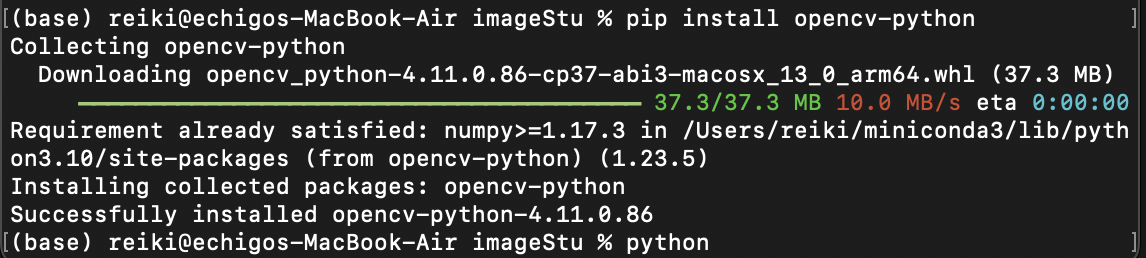
\includegraphics[width=10cm]{install_screenshot.png}
    \caption{OpenCVインストール時の画面}
\end{figure}

\section*{(3) 実行準備:読み込み・描画コードの動作確認}

\subsection*{(1) 画像の読み込み・表示コード}

\begin{lstlisting}[caption=画像表示のコード]
import cv2

img = cv2.imread("report1/testImage.jpg.webp")
cv2.imshow("Image", img)
cv2.waitKey(0)
cv2.destroyAllWindows()
\end{lstlisting}

図2に実行結果画面を示す。

\begin{figure}[H]
    \centering
    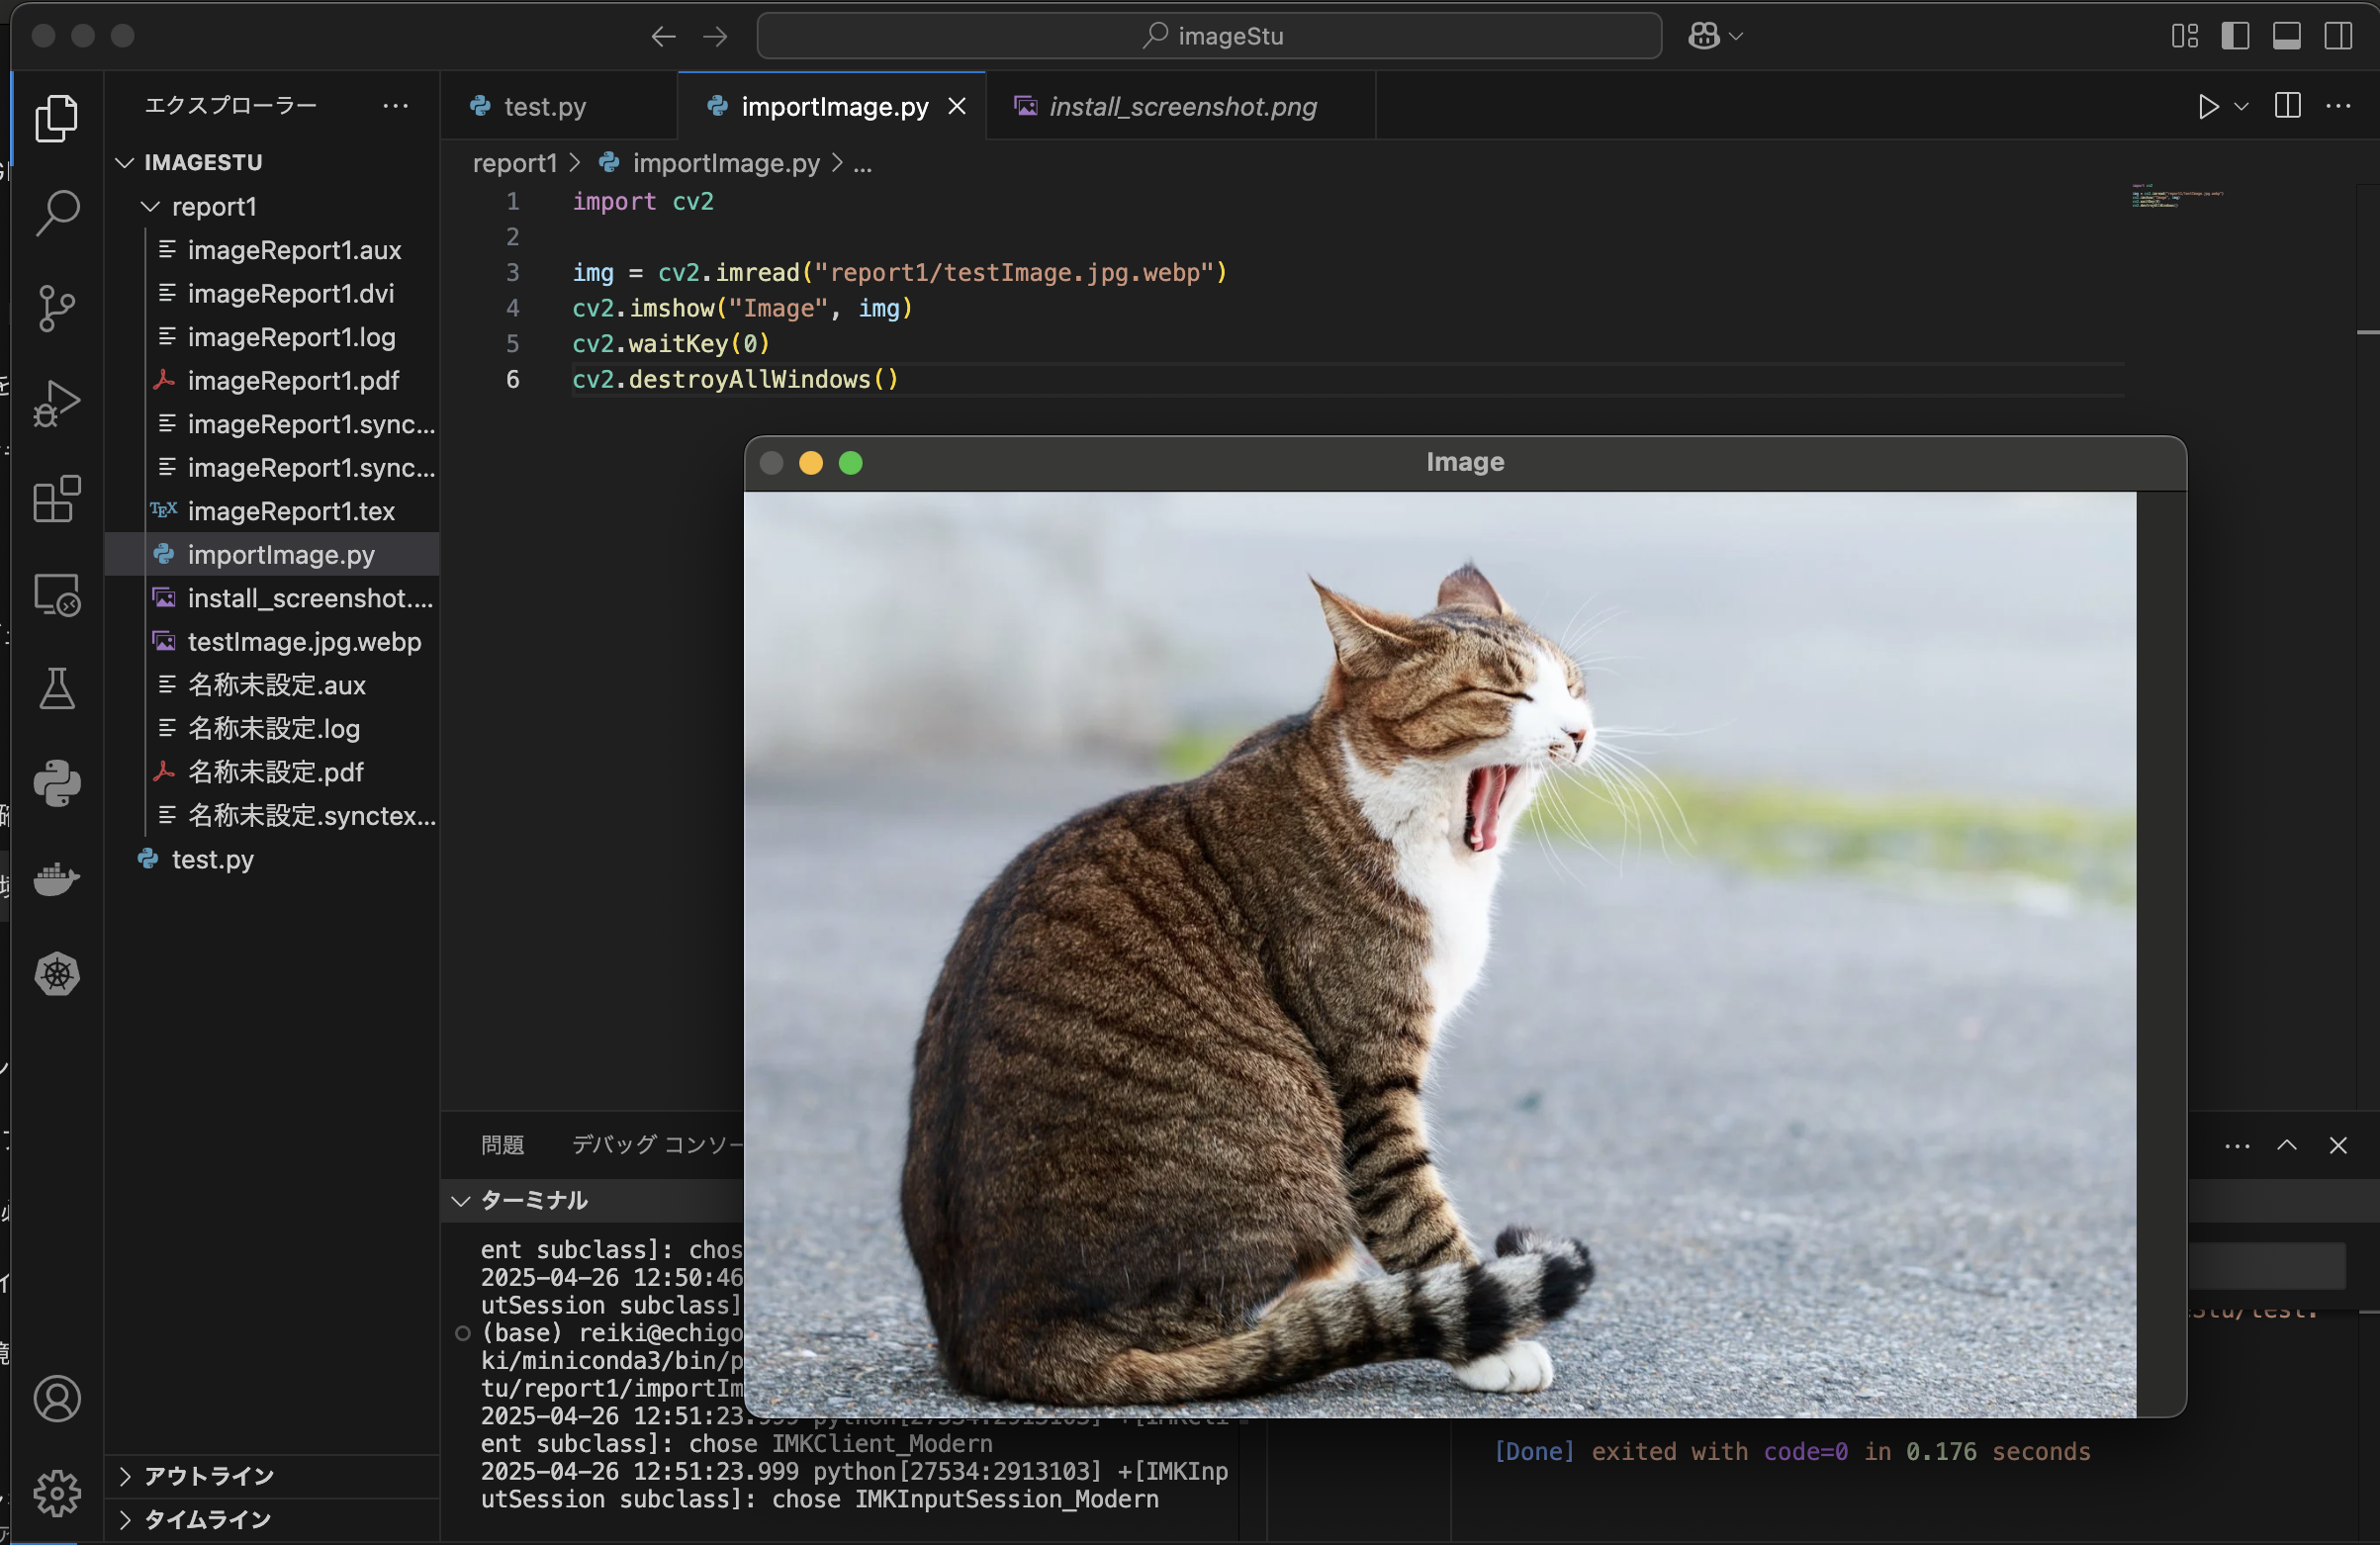
\includegraphics[width=10cm]{test_screenshot.png}
    \caption{実行時画面(画像表示)}
\end{figure}

\subsection*{(2) 図形・文字の描画コード}

\begin{lstlisting}[caption=図形・文字の描画コード]
import cv2
import numpy as np

img = np.zeros((500, 500, 3), dtype=np.uint8)

cv2.line(img, (50, 50), (450, 50), (255, 0, 0), 3)
cv2.rectangle(img, (50, 100), (200, 200), (0, 255, 0), -1)
cv2.circle(img, (300, 300), 50, (0, 0, 255), -1)
cv2.putText(img, "Hello OpenCV", (100, 400),
            cv2.FONT_HERSHEY_SIMPLEX, 1, (255, 255, 255), 2)

cv2.imshow("Drawing", img)
cv2.waitKey(0)
cv2.destroyAllWindows()
\end{lstlisting}

図3に実行結果画面を示す。

\begin{figure}[H]
    \centering
    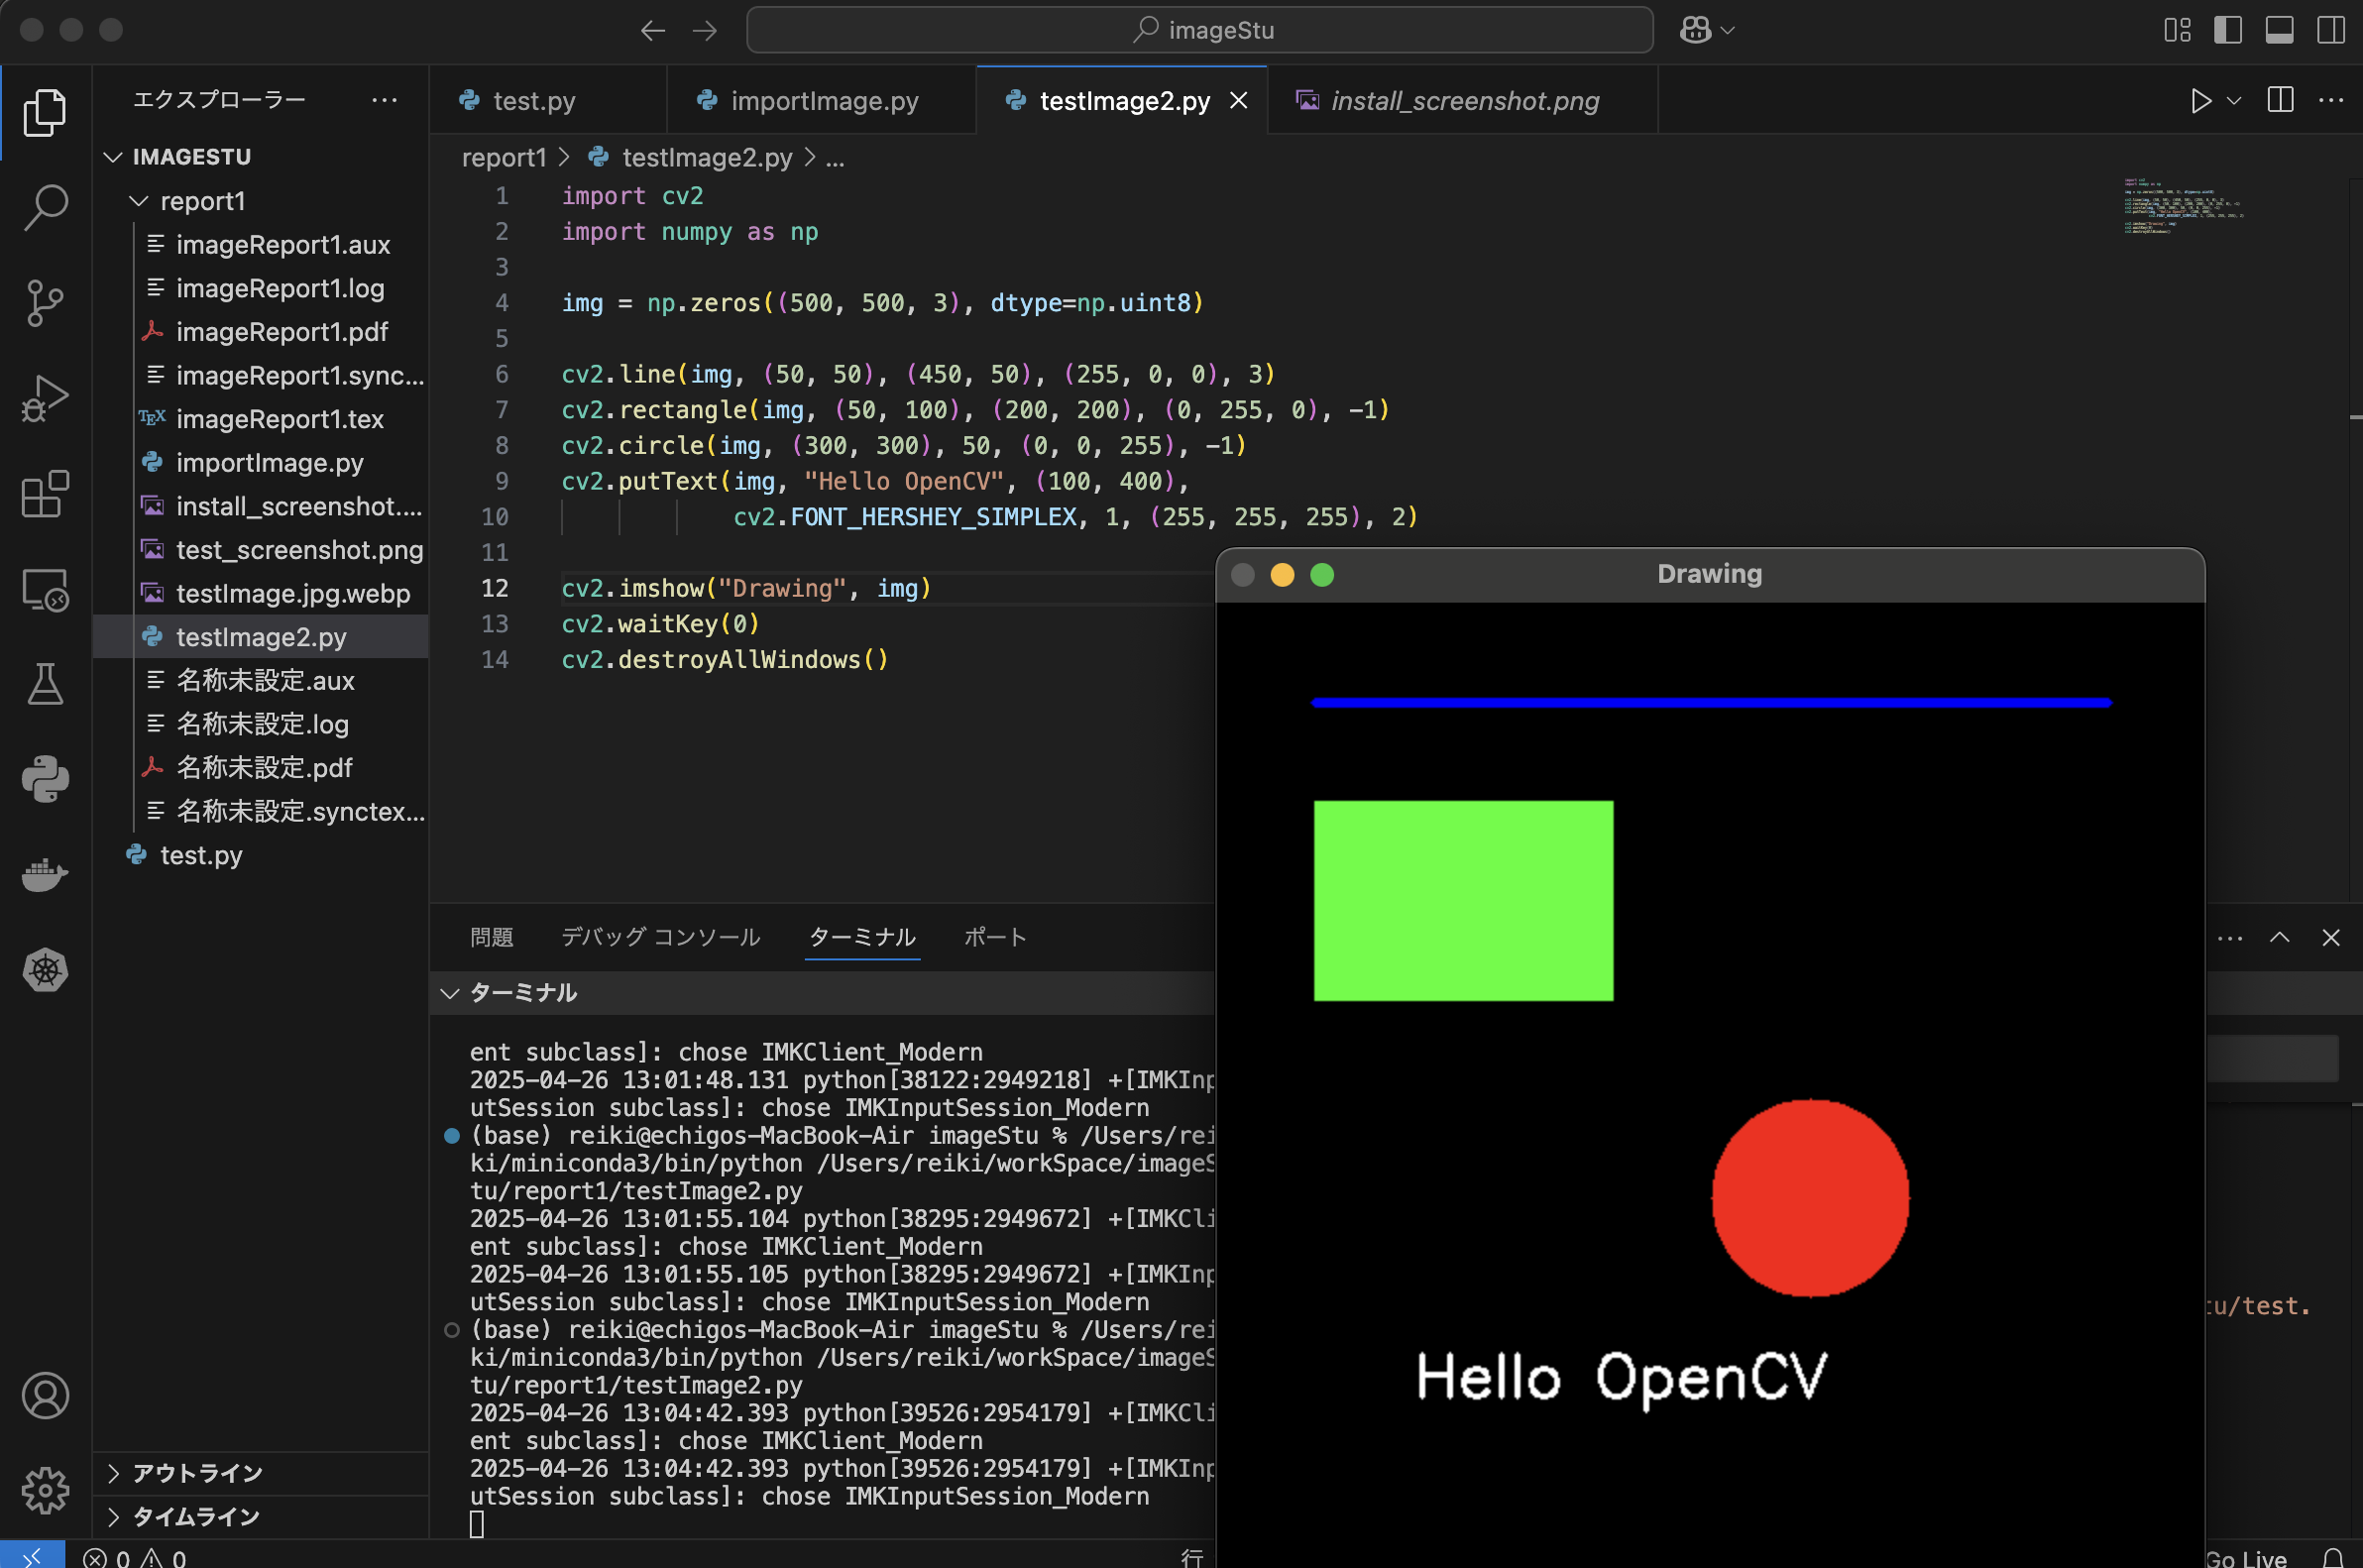
\includegraphics[width=10cm]{test_screenshot2.png}
    \caption{実行時画面(図形・文字描画)}
\end{figure}

\end{document}
